%%%%%%%%%%%%%%%%%%%%%%%%%%%%%%%%%%%%%%%%%%%%%%%%%%%%%%%%%%%%%%%%%%%%%%%%%%%%%%%
\chapter{Ondas estacionárias}
\label{Chap:ExpOndasEstacionarias}
%%%%%%%%%%%%%%%%%%%%%%%%%%%%%%%%%%%%%%%%%%%%%%%%%%%%%%%%%%%%%%%%%%%%%%%%%%%%%%%

\begin{fullwidth}\it
Submeteremos um fio a uma tensão e a uma vibração, com a consequente formação de ondas estacionárias. O objetivo desse experimento é verificarmos experimentalmente as propriedades de tais ondas e as relações com os diversos parâmetros do sistema. Utilizaremos os seguintes conceitos/técnicas de análise de dados: medidas, algarismos significativos, gráficos, software para elaboração de gráficos, erros de escala e propagados, equação geral para o erro propagado, regressão linear, linearização, e erros dos coeficientes $A$ e $B$.
\end{fullwidth}

%%%%%%%%%%%%%%%%%%%%%%%%%%%%%%%%%%%%%%%%%%%%%%%%%%%%%%%%%%%%%%%%%%%%%%%%%%%%%%%
\section{Ondas transversais}
%%%%%%%%%%%%%%%%%%%%%%%%%%%%%%%%%%%%%%%%%%%%%%%%%%%%%%%%%%%%%%%%%%%%%%%%%%%%%%%

\begin{marginfigure}[5cm]
\centering
\begin{tikzpicture}[>=Stealth,domain=0:3.1415,samples=50]
	\draw[->] (-0.5,0) -- (4,0) node[below]{$x$};
	\draw[<-] (0,1.5) node[left]{$y$} -- (0,-1.5);
	\draw[color = black,smooth] plot (\x,{sin(2 * \x r)});
	
	\draw[dotted] (3.1415,-1.2) -- (3.1415,0);
	\draw[<->] (0,-1.2) -- node[below]{$\lambda$} (3.1415,-1.2);
	\draw[<->] (0.7854,0) -- node[right]{$A$} (0.7854,1);
\end{tikzpicture}
\caption{Parâmetros espaciais de uma onda transversal.}
\label{Fig:OndaCongelada}
\end{marginfigure}

\begin{marginfigure}
\centering
\begin{tikzpicture}[>=Stealth,domain=0:3.1415,samples=50]
	\draw[->] (-0.5,0) -- (4,0) node[below]{$t$};
	\draw[<-] (0,1.5) node[left]{$y$} -- (0,-1.5);
	\draw[color = black,smooth] plot (\x,{sin(2 * \x r)});
	
	\draw[dotted] (3.1415,-1.2) -- (3.1415,0);
	\draw[<->] (0,-1.2) -- node[below]{$T$} (3.1415,-1.2);
	\draw[<->] (0.7854,0) -- node[right]{$A$} (0.7854,1);
\end{tikzpicture}
\caption{Parâmetros temporais de uma onda transversal.}
\label{Fig:OscilacaoPontoOnda}
\end{marginfigure}

Uma onda mecânica é uma perturbação periódica que se propaga em um meio. No caso de uma onda transversal, tal perturbação é um deslocamento lateral, perpendicular à direção de propagação da onda. Esse tipo de onda pode ser descrita como uma função $y(x,t)$, onde $y$ representa o valor da perturbação na posição $x$ e tempo $t$. A forma mais simples para essa função é
\begin{equation}\label{Eq:OndaUnidimensional}
	y(x,t) = A \sen(kx - \omega t),
\end{equation}
%
onde $A$ é a amplitude da onda ---~isto é, o valor máximo atingido pela variável $y$~--- e os parâmetros $k$ e $\omega$ são denominados como \emph{número de onda} e \emph{frequência angular}, respectivamente.

Tal expressão pode ser entendida de maneira simples se considerarmos dois casos especiais: $x = 0$ para qualquer $t$ e $t = 0$ para qualquer $x$. Isso resulta nas expressões
\begin{equation}
	y(t) = A \sen (\omega t),
\end{equation}
%
e
\begin{equation}
	y(x) = A \sen(kx).
\end{equation}
%
O primeiro caso representa simplesmente a oscilação de um ponto do meio no qual a onde se propaga (especificamente, nesse caso, aquele localizado na origem do eixo $x$). No segundo caso, temos uma análise de toda a onda em um dado instante de tempo, como se a congelássemos (veja a Figura~\ref{Fig:OndaCongelada}).

%%%%%%%%%%%%%%%%%%%%%%%%%%%%%%%%%%%%%%%%%%%%%%%%%%%%%%%%%%%%%
\paragraph{Interpretação da frequência angular para uma onda}
%%%%%%%%%%%%%%%%%%%%%%%%%%%%%%%%%%%%%%%%%%%%%%%%%%%%%%%%%%%%%

Sabemos que o a função $\sen \theta$ se repete a partir de $\theta = 2\pi$, o que se reflete em uma repetição do movimento oscilatório. Consequentemente, temos que ao final de uma oscilação
\begin{equation}
	\omega T = 2 \pi,
\end{equation}
%
onde usamos $t = T$ ---~isto é, a variável $t$ assume o valor do período $T$ da oscilação (o tempo que o movimento oscilatório demora para completar um ciclo)~---. Logo
\begin{equation}
	\omega = \frac{2 \pi}{T}.
\end{equation}
%
Para determinarmos o número de oscilações por unidade de tempo ---~a frequência da oscilação~---, basta dividirmos uma unidade de tempo pela duração de uma oscilação, ou seja,
\begin{equation}
	f = \frac{1}{T},
\end{equation}
%
o que nos permite escrever
\begin{equation}
	\omega = 2 \pi f.
\end{equation}

%%%%%%%%%%%%%%%%%%%%%%%%%%%%%%%%%%%%%%%%%%%
\paragraph{Interpretação do número de onda}
%%%%%%%%%%%%%%%%%%%%%%%%%%%%%%%%%%%%%%%%%%%

Se nos deslocamos na direção do eixo $x$, observamos uma variação da posição $y$, sendo que após percorrermos uma distância $\lambda$ ---~denominada \emph{comprimento de onda}~--- o movimento se repete. Novamente, como a função $\sen\theta$ se repete após $\theta = 2\pi$, temos que para a posição $x = \lambda$
\begin{equation}
	k \lambda = 2\pi,
\end{equation}
%
ou
\begin{equation}
	k = \frac{2\pi}{\lambda}.
\end{equation}

%%%%%%%%%%%%%%%%%%%%%%%%%%%%%%%%%%%%%%%%%%%%%%%%
\paragraph{Velocidade de propagação de uma onda}
%%%%%%%%%%%%%%%%%%%%%%%%%%%%%%%%%%%%%%%%%%%%%%%%

Podemos calcular a velocidade de propagação da onda simplesmente verificando que uma crista qualquer (o ponto em que $y$ atinge o valor máximo) se desloca uma distância $\lambda$ a cada oscilação. Logo
\begin{equation}\label{Eq:RelVelFreqAngNumOnda}
	v = \frac{\lambda}{T} = \lambda f = \frac{\omega}{k}.
\end{equation}
%
A velocidade de propagação de uma onda é uma constante que depende de características do meio no qual a onda se propaga. Em uma onda transversal em uma corda, por exemplo, ela é dada por
\begin{equation}\label{Eq:VelocidadeOndaEmUmaCorda}
    v = \sqrt{\frac{T}{\mu}},
\end{equation}
%
onde $T$ representa a tensão a qual a corda está submetida, e $\mu$ representa a densidade linear de massa da corda. Portanto, os valores da frequência angular $\omega$ e do número de onda $k$ não são independentes, pois estão ligados através da velocidade.

%%%%%%%%%%%%%%%%%%%%%%%%%%%%%%%%%%%%%%%%%%%%%
\paragraph{Sentido de propagação de uma onda}
%%%%%%%%%%%%%%%%%%%%%%%%%%%%%%%%%%%%%%%%%%%%%

O sentido de propagação da onda está ligado ao sinal do termo $\omega t$ na Equação~\eqref{Eq:OndaUnidimensional}. Podemos entender tal relação, consideramos um sistema de referência ortogonal $xy$ e uma onda que se propaga no sentido positivo do eixo $x$, como mostrado na Figura~\ref{Fig:SinalPropOndaSentidoPositivo}. No referencial $xy$, a onda é descrita através de uma função $y(x,t)$ e se propaga com velocidade $v$.

\begin{marginfigure}
\centering
\begin{tikzpicture}[>=Stealth]

    \draw[densely dotted, ->] (-0.5,0) -- (3.5,0) node[below left]{$x$};
    \draw[densely dotted, ->] (0,-1.5) -- (0,1.5) node[below left]{$y$};
    
	\draw[smooth, domain=-0.5:3.2,samples=50] plot (\x,{sin(2 * \x r)});
    
    \draw [->] (1.25,0) -- (2.75,0) node[above left]{$x'$};
    \draw [->] (1.25,0) -- (1.25,1.25) node[left]{$y'$};

    \draw [dotted] (1.25,0) -- (1.25, -0.5);    
    \draw [|<->|] (0, -0.5) -- node[below]{$v\cdot t$} (1.25, -0.5);
    
    \draw[->] (1.25, 1) -- (2,1) node[above]{$\vec{v}$};

\end{tikzpicture}
\caption{Para uma onda que se propagan no sentido positivo de $x$, a relação entre as coordenadas $x$ e $x'$ é $x' = x - vt$.\label{Fig:SinalPropOndaSentidoPositivo}}
\end{marginfigure}

Em um segundo referencial ortogonal, denotado $x'y'$, que se move na direção e sentido do eixo $x$, com velocidade $v$ em relação ao primeiro sistema de referência, temos que a velocidade da onda é nula. A função $y'$ que descreve a onda deve então depender somente da posição $x'$ nesse referencial, ou seja, temos somente $y'(x')$. Podemos assumir que no referencial $x'y'$ a expressão para a onda é dada por
\begin{equation}
    y'(x') = A\sen(kx').
\end{equation}
%
A relação entre $x'$ e $x$ é dada por
\begin{equation}
    x' = x - vt,
\end{equation}
%
portanto, podemos escrever $y'(x,t)$ como
\begin{align}
    y'(x,t) &= A\sen(k[x - vt]) \\
    &= A\sen(kx - kvt).
\end{align}    

Considerando que a origem dos eixos $y$ e $y'$ coincide, podemos escrever $y'(x,t) = y(x,t)$, o que nos permite escrever
\begin{equation}
    y(x,t) = A\sen(kx - \omega t), \mathnote{Onda transversal que se propaga no sentido positivo}
\end{equation}
%
onde utilizamos a Equação~\ref{Eq:RelVelFreqAngNumOnda} para eliminar a velocidade. Note, portanto, que no caso em que a onda se desloca no sentido \emph{positivo}, o sinal deve ser \emph{negativo}.

\begin{marginfigure}[3cm]
\centering
\begin{tikzpicture}[>=Stealth]

    \draw[densely dotted, ->] (-0.5,0) -- (3.5,0) node[below left]{$x$};
    \draw[densely dotted, ->] (2.5,-1.5) -- (2.5,1.5) node[below left]{$y$};
    
	\draw[smooth, domain=-0.5:3.2,samples=50] plot (\x,{sin(2 * \x r)});
    
    \draw [->] (0.4,0) -- (1.5,0) node[below left]{$x'$};
    \draw [->] (0.4,0) -- (0.4,1.25) node[left]{$y'$};

    \draw [dotted] (0.4,0) -- (0.4, -0.5);    
    \draw [|<->|] (0.4, -0.5) -- node[below]{$v\cdot t$} (2.5, -0.5);
    
    \draw[->] (0.4, 1) -- (-0.1,1) node[below]{$\vec{v}$};

\end{tikzpicture}
\caption{No caso de uma onda que se propagan no sentido negativo de $x$, a relação entre as coordenadas $x$ e $x'$ é $x' = x + vt$.\label{Fig:SinalPropOndaSentidoNegativo}.}
\end{marginfigure}

Caso a onda se desloque no sentido negativo do eixo $x$, novamente com um sistema de referência ortogonal $x'y'$ que se move na mesma direção e sentido para a qual a onda se propaga ~---como mostrado na Figura~\ref{Fig:SinalPropOndaSentidoNegativo}~---, temos como única diferença o fato de que a relação entre $x'$ e $x$ é dada por
\begin{equation}
    x' = x + vt,
\end{equation}
%
de onde obtemos
\begin{equation}
    y(x,t) = A\sen(kx + \omega t). \mathnote{Onda transversal que se propaga no sentido negativo}
\end{equation}
%
Portanto, se a onda se desloca no sentido \emph{negativo} do eixo $x$, temos um sinal \emph{positivo}.

\begin{marginfigure}[2cm]
\centering
\begin{tikzpicture}[>=Stealth]

    \draw[->] (0,0) -- (4,0) node[below left]{$x$};
    \draw[->] (0,-1.5) -- (0,1.5) node[below left]{$y$};
    
    \draw (1.4,0) -- +(0,1);
    \draw (0.8,0.6754) -- +(1,0);
	\draw[smooth, domain=0:3.1415,samples=50] plot (\x,{sin(2 * \x r)});
    \draw[fill] (1.4,0.335) circle (1pt);
    \draw[fill = white, draw = black] (1.2,0.6754) circle (1pt);
    
	\draw[smooth, dotted, domain=0:3.1415,samples=50] plot (\x,{sin(2 * (\x - 0.2) r)});
	
	\draw[fill = white, draw = black] (1.4,0.6754) circle (1pt);
     	
\end{tikzpicture}
\caption{Ao aumentarmos o valor de $t$, temos uma diminuição do valor do argumento da função seno. Poderíamos ter uma diminuição equivalente reduzindo o valor de $x$, o que equivale a alterar a posição do ponto preenchido para o ponto vazado. Tal alteração equivale, por sua vez, a deslocar todo o gráfico para a direita.}
\end{marginfigure}

Uma maneira alternativa de compreender a relação entre o sinal e o sentido de propagação é a de que se tomarmos um valor de $x$ qualquer com um valor de $\sen(kx-\omega t)$ correspondente, quando $t$ aumenta, o valor do argumento ---~isto é, $kx -\omega t$~--- diminui. Equivalentemente, poderíamos simplesmente diminuir o argumento escolhendo um valor de $x$ menor, ou seja, escolheríamos um ponto à esquerda. O efeito de aumentar o $t$ é então o de tomar o ``gráfico'' do $\sen(kx)$ e deslocá-lo para a direita, o que implica em uma propagação da onda para a direita. Logo, para uma onda que se propaga no sentido positivo
\begin{equation}
    y(x,t) = A\sen(kx -\omega t).
\end{equation}

\begin{figure*}[t]
\centering
\forceversofloat
\begin{tikzpicture}[>=Stealth,domain=0:13,samples=250]
	\draw[<-] (0,2) node[left]{$y$} -- (0,-2);
	\draw[color = gray!05,smooth,thick] plot (\x,{1.7 * sin(\x r)});
	\draw[color = gray!10,smooth,thick] plot (\x,{1.7 * sin((\x - 0.1) r)});
	\draw[color = gray!20,smooth,thick] plot (\x,{1.7 * sin((\x - 0.2) r)});
	\draw[color = gray!40,smooth,thick] plot (\x,{1.7 * sin((\x - 0.3) r)});
	\draw[color = gray!60,smooth,thick] plot (\x,{1.7 * sin((\x - 0.4) r)});
	\draw[color = gray!80,smooth,thick] plot (\x,{1.7 * sin((\x - 0.5) r)});
	\draw[color = gray,smooth,thick] plot (\x,{1.7 * sin((\x - 0.6) r)});		
	\draw[color = black,smooth,thick] plot (\x,{1.7 * sin((\x - 0.7) r)});
	\draw[->] (-0.5,0) -- (15,0) node[below]{$x$};
\end{tikzpicture}
\caption{Evolução temporal de uma onda transversal descrita por $y(x,t) = A \sen(kx - \omega t)$.}
\label{Fig:Onda}
\end{figure*}

%%%%%%%%%%%%%%%%%%%%%%%%%%%%%%%%
\subsection{Ondas estacionárias}
%%%%%%%%%%%%%%%%%%%%%%%%%%%%%%%%

Vamos supor que duas ondas com os mesmos valores de amplitude $A$, frequência angular $\omega$, e número de onda $k$, se propagam em sentidos opostos em um mesmo meio\footnote[][-1cm]{Uma maneira simples de se obter tal fenômeno é utilizar uma corda presa a uma parede e em cuja extremidade livre ligamos um oscilador (cuja função é gerar a perturbação, ou seja, a onda). Ao se propagar, a onda atinge a extremidade fixa e é refletida, passando a trafegar no sentido oposto, o que faz com que ela interfira com pulsos de onda gerados posteriormente, e que ainda estão se propagando no sentido original.}. Podemos descrever tais ondas através das expressões
\begin{align}
	y_1(x,t) &= A \sen(kx - \omega t) \\
	y_2(x,t) &= A \sen(kx + \omega t).
\end{align}
%
Quando ambas estiverem se propagando em uma mesma região do meio de propagação, a onda resultante será dada por:\footnote[][2cm]{O fato de que as perturbações devido a ondas diferentes se somam é conhecido como \emph{princípio da superposição} e sua origem reside no fato de que o meio apresenta uma resposta linear a perturbações.}
\begin{align}
	y_{1+2}(x,t) &= y_1(x,t) + y_2(x,t)\\
	&= A \sen(kx -\omega t) + A \sen(kx + \omega t).
\end{align}
%
Utilizando a propriedade
\begin{equation}
	\sen \alpha + \sen \beta = 2 \sen[(\alpha + \beta)/2]\cos[(\alpha-\beta)/2],
\end{equation}
podemos reescrever a superposição das duas ondas como
\begin{equation}\label{Eq:EqOndaEstacionaria}
	y_{1+2}(x,t)=[2A\sen kx]\cos\omega t.
\end{equation}

\begin{figure*}[b]\forceversofloat
\centering
\begin{tikzpicture}[>=Stealth,domain=0:13,samples=250]
	\draw[->] (-0.5,0) -- (15,0) node[below]{$x$};
	\draw[<-] (0,2) node[left]{$y$} -- (0,-2);
	\draw[color = gray!05,smooth,thick] plot (\x,{1.7 * sin(\x r) * cos(2.3 r)});
	\draw[color = gray!10,smooth,thick] plot (\x,{1.7 * sin(\x r) * cos(2.1 r)});
	\draw[color = gray!20,smooth,thick] plot (\x,{1.7 * sin(\x r) * cos(1.9 r)});
	\draw[color = gray!40,smooth,thick] plot (\x,{1.7 * sin(\x r) * cos(1.7 r)});
	\draw[color = gray!60,smooth,thick] plot (\x,{1.7 * sin(\x r) * cos(1.5 r)});
	\draw[color = gray!80,smooth,thick] plot (\x,{1.7 * sin(\x r) * cos(1.3 r)});
	\draw[color = gray,smooth,thick] plot (\x,{1.7 * sin(\x r) * cos(1.1 r)});		
	\draw[color = black,smooth,thick] plot (\x,{1.7 * sin(\x r) * cos(0.7 r)});
	\draw[dashed,color=gray] plot (\x,{1.7 * sin(\x r)});
	\draw[dashed,color=gray] plot (\x,{-1.7 * sin(\x r)});
\end{tikzpicture}
\caption{Evolução temporal de uma onda transversal estacionária.}
\label{Fig:OndaEstacionaria}
\end{figure*}

Na Equação~\eqref{Eq:EqOndaEstacionaria}, o termo entre colchetes denota a amplitude de uma onda cuja posição no eixo $y$ muda com o tempo conforme $\cos\omega t$. Analisando tal expressão, percebemos que para valores periódicos de $x$, o valor da amplitude é \emph{zero}. Isso implica que, no caso da superposição das duas ondas, temos uma onda resultante na qual alguns pontos (denominados \emph{nós}) permanecem parados, enquanto os demais pontos variam sua posição com o tempo, sendo que a amplitude dessa oscilação depende da posição em $x$. Podemos verificar na Figura~\ref{Fig:OndaEstacionaria} uma onda estacionária descrita por tal equação. A linha em preto mostra o estado atual, enquanto as demais mostram o estado da onda em instantes anteriores (em intervalos regulares de tempo). Note que existem ``ventres'' delimitados por $\pm 2A\sen kx$ (linhas tracejadas), isto é, ventres cujo perfil é dado pela função $2A\sen kx$ tanto acima, quanto abaixo da direção de propagação $x$. Portanto, o movimento da onda fica restrito a deslocamentos na direção do eixo $y$, limitado pelas linhas tracejadas.

De acordo com o termo $[2A\sen kx]$, a posição dos nós pode ser obtida fazendo com que
\begin{equation}
	kx = n\pi.
\end{equation}
%
onde $n = 0, 1, 2, 3, \dots$, isto é, um número inteiro não negativo. Substituindo a expressão para o número de onda $k = (2\pi)/\lambda$, obtemos
\begin{equation}
	x = n \frac{\lambda}{2}.
\end{equation}
%
Temos então que, para uma onda estacionária, os nós aparecem a cada meio comprimento de onda.

%%%%%%%%%%%%%%%%%%%%%%%%%%%%%%%%%%%%%%%%%%%%%%%%%%%%%%%%%%%%%%%%
\section{Ondas estacionárias em uma corda fixada em dois pontos}
%%%%%%%%%%%%%%%%%%%%%%%%%%%%%%%%%%%%%%%%%%%%%%%%%%%%%%%%%%%%%%%%

Em uma onda estacionária, os pontos de fixação devem ser obrigatoriamente nós (afinal, para que houvesse um ventre nos pontos de fixação, a corda precisaria oscilar, o que a fixação impede). Isso faz com que tenhamos um \emph{número inteiro de meios comprimentos de onda} entre os pontos de fixação. Como a velocidade da onda no meio é uma constante característica do próprio meio, concluímos que somente algumas frequências específicas são capazes de gerar ondas estacionárias.

Sabemos que a amplitude da onda estacionária será nula sempre que
\begin{equation}
	kx = n\pi,
\end{equation}
%
logo, os dois primeiros nós são então em $x=0$ e em $x = \lambda/2$. Isto significa que temos uma onda estacionária de forma que a distância entre os pontos de fixação equivale a \emph{meio comprimento de onda}.

Temos outras possibilidades, no entanto: se assumirmos que no segundo ponto de fixação temos o terceiro nó, temos que a distância entre os pontos de fixação será coberta por dois ventres (um comprimento de onda). De forma geral temos que a distância $L$ entre os pontos de fixação é igual a um número inteiro de meios comprimentos de onda:
\begin{equation}\label{Eq:RelComprimentoCordaEComprimentosDeOndaNaRessonancia}
    L = n'\frac{\lambda}{2}.
\end{equation}
%
O valor de $n' = 1, 2, 3, \dots$ designa o número\footnote{O número de ventres $n'$ está relacionado ao número de nós $n$ por $n'=n-1$.} de ventres da onda estacionária. Como a frequência está relacionada com a velocidade $v$ e o comprimento de onda através de
\begin{equation}
	f = \frac{v}{\lambda},
\end{equation}
%
para uma onda estacionária temos que,
\begin{equation}\label{Eq:RelacaoVariaveisOndasEstacionarias}
	f = \frac{n'}{2L}\sqrt{\frac{T}{\mu}},
\end{equation}
%
onde utilizamos as Equações~\eqref{Eq:VelocidadeOndaEmUmaCorda} e~\eqref{Eq:RelComprimentoCordaEComprimentosDeOndaNaRessonancia}.\footnote{No aparato experimental adotado, a corda passa por uma polia e sustenta um conjunto de anilhas. A tensão na corda será então igual ao peso do conjunto, isto é, $T = mg$.}

Portanto, é interessante notar que para uma corda cujas extremidades são fixas existem múltiplos ---~porém específicos~--- valores de frequência para os quais podemos ter uma onda estacionária. Essas frequências são denominadas \emph{frequências de ressonância}, sendo que a menor delas é denominada \emph{modo fundamental} ou \emph{frequência fundamental} ---~ou ainda, \emph{primeiro harmônico}~---, enquanto as demais são denominadas \emph{segundo harmônico} ($n'=2$), \emph{terceiro harmônico} ($n'=3$), etc.

%%%%%%%%%%%%%%%%%%%%%%%%%%%%%%%%%%%%%%%%%%%%%%%%%%%%%%%%%%%%%%%%%%%%%%%%%%%%%%%
\section{Experimento}
%%%%%%%%%%%%%%%%%%%%%%%%%%%%%%%%%%%%%%%%%%%%%%%%%%%%%%%%%%%%%%%%%%%%%%%%%%%%%%%

%%%%%%%%%%%%%%%%%%%%%%
\subsection{Objetivos}
\label{Sec:ObjetivosOndasEstacionarias}
%%%%%%%%%%%%%%%%%%%%%%

\begin{itemize}
	\item Verificar a proporcionalidade da frequência de ressonância $f$ com a raiz quadrada da tensão exercida pela corda, sendo que a tensão será variada ao se alterar a massa $m$ suspensa na extremidade livre;
	\item Linearizar a equação que relaciona a frequência à massa, determinando a função $F_1(m)$ de forma que um gráfico $f \times F_1(m)$ seja linear.
	\item Verificar a proporcionalidade da frequência de ressonância $f$ com o inverso do comprimento $L$ da corda.
	\item Linearizar a equação que relaciona a frequência ao comprimento, determinando a função $F_2(L)$ de forma que um gráfico $f \times F_2(L)$ seja linear.
	\item Determinar o valor da densidade linear de massa através do coeficiente angular dos gráficos $f \times F_2(L)$.
	\item Determinar o valor da gravidade através do coeficiente angular dos gráficos $f \times F_1(m)$.
\end{itemize}

\begin{figure}\forcerectofloat
	\centering
	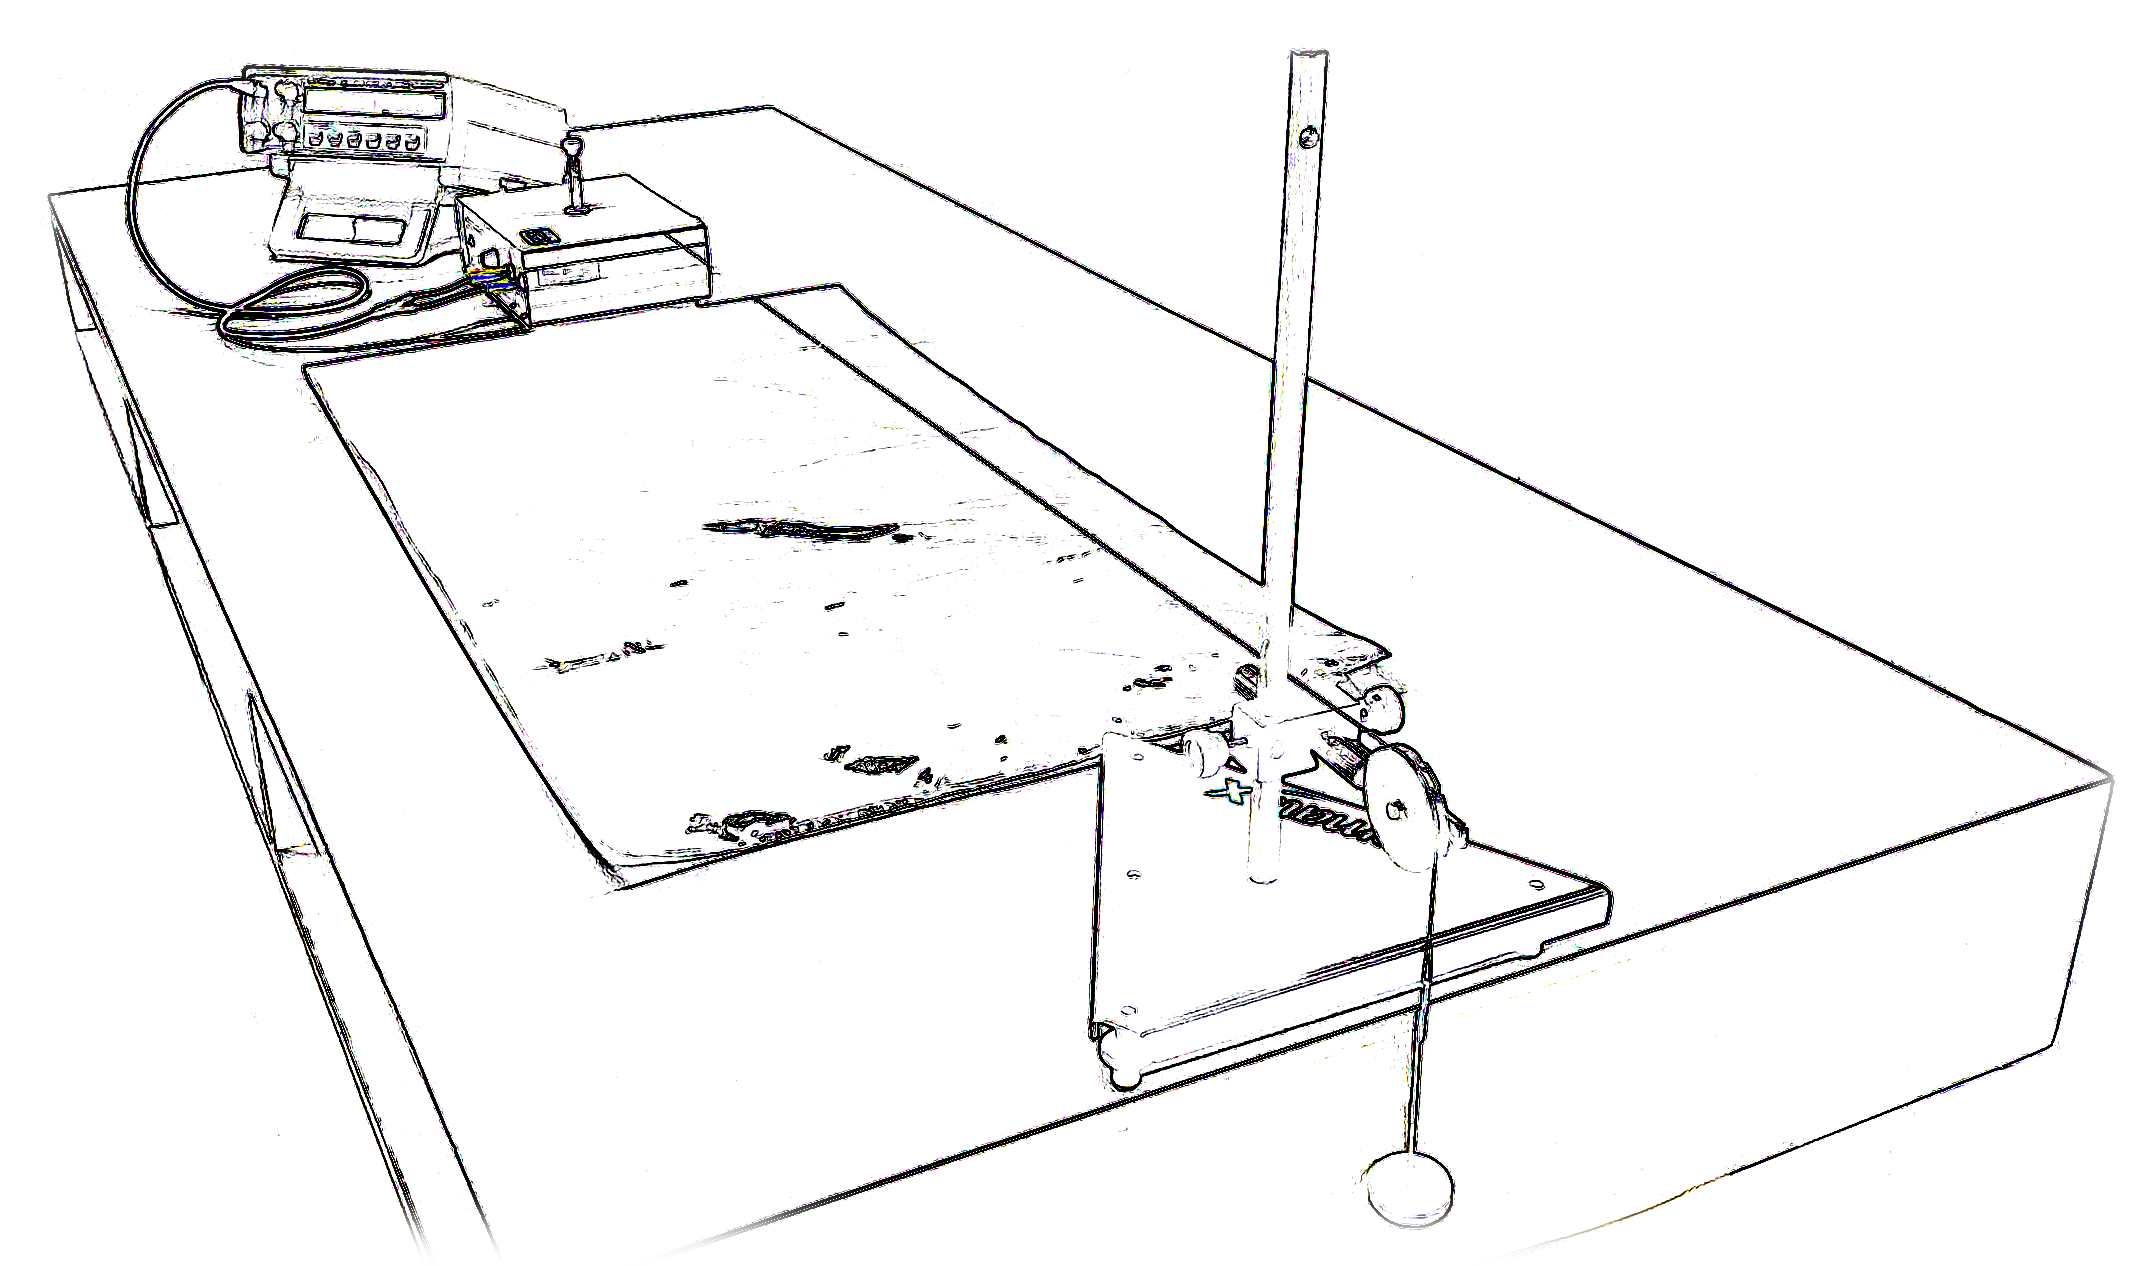
\includegraphics[width=\textwidth]{Ilustrations/Ondas_estacionarias.png}
	\caption{Aparato para a visualização de ondas estacionárias em uma corda.}
\end{figure}

%%%%%%%%%%%%%%%%%%%%%%%%%%%%%%%%%%%%%%%%%%%%%%%%%%%%%%%%%%%%%%%%%%%%%%%%%%%%%%%
\section{Material Necessário}
%%%%%%%%%%%%%%%%%%%%%%%%%%%%%%%%%%%%%%%%%%%%%%%%%%%%%%%%%%%%%%%%%%%%%%%%%%%%%%%

\begin{itemize}
	\item Gerador de ondas;
	\item Trena;
	\item Fio fino;
	\item Balança;
	\item Anilhas leves e gancho;
	\item Polia com suporte.
\end{itemize}

%%%%%%%%%%%%%%%%%%%%%%%%%%%%%%%%%%%%%%%%%%%%%%%%%%%%%%%%%%%%%%%%%%%%%%%%%%%%%%%
\section{Procedimento Experimental}
%%%%%%%%%%%%%%%%%%%%%%%%%%%%%%%%%%%%%%%%%%%%%%%%%%%%%%%%%%%%%%%%%%%%%%%%%%%%%%%

%%%%%%%%%%%%%%%%%%%%%%%%%%%%%%%%%%%%%%%%%%%%%%%%%%%%%%%%%%%%%%%%%%%%%%%%
\subsection{Determinação da densidade linear de massa do fio (opcional)}
%%%%%%%%%%%%%%%%%%%%%%%%%%%%%%%%%%%%%%%%%%%%%%%%%%%%%%%%%%%%%%%%%%%%%%%%

O valor de densidade de massa do fio utilizado pode ser determinado com a utilização de uma balança de alta precisão. Para isso basta tomarmos um segmento com um comprimento $L$ arbitrário, porém determinado, e verificarmos qual a massa $m$ correspondente. Obtemos a densidade linear de massa $\mu$ através da razão
\begin{equation}
	\mu = \frac{m}{L}.
\end{equation}
%
O valor obtido dessa forma será considerado o \emph{valor de referência} na análise de dados.

%%%%%%%%%%%%%%%%%%%%%%%%%%%%%%%%%%%%%%%%%%%%%%%%%%%%%%%%%%%%%%%%%%%%%%%%%%%
\subsection{Dependência da frequência de ressonância com a tensão aplicada}
%%%%%%%%%%%%%%%%%%%%%%%%%%%%%%%%%%%%%%%%%%%%%%%%%%%%%%%%%%%%%%%%%%%%%%%%%%%

\begin{enumerate}
\item Ligue o gerador de ondas ao oscilador eletromecânico, dispondo o segundo a uma distância de aproximadamente \np[m]{1,30} da extremidade da mesa;\label{Enum:iteminicio}
\item Prenda a polia ao suporte e a disponha de forma que fique para fora da mesa.
\item Tome um segmento de fio com tamanho adequado e o prenda ao pino do oscilador. Anote na Tabela~\ref{Tab:FrequenciaFuncaoMassa} o valor de referência para densidade linear de massa $\mu$ do fio utilizado;
\item Afira a massa do gancho, juntamente com uma anilha e os pendure na extremidade livre da corda, fazendo-a passar pela polia e deixando o gancho suspenso. Anote na Tabela~\ref{Tab:FrequenciaFuncaoMassa} o valor da massa $m$ suspensa na corda;\label{Enum:itemfim}
\item Ligue o gerador de ondas e varie a frequência até que se forme uma onda estacionária com dois\footnote{Esse harmônico foi escolhido por ser o de mais fácil visualização.} ventres ($n' =2$);
\item Anote o valor da frequência $f$ em que a onda estacionária se forma na Tabela~\ref{Tab:FrequenciaFuncaoMassa}. \emph{Obs.: Em alguns equipamentos, a frequência pode variar constantemente. Nesse caso, anote os valores com uma casa após a vírgula e adote o valor de erro como sendo \np[Hz]{0,1}.}
\item Utilize a trena/régua para medir a distância $L$ entre \emph{os nós das extremidades}\footnote{A distância deve ser medida entre o ponto em que a corda toca a polia (onde se localiza um dos nós) e o nó que deve se formar um pouco antes do pino do oscilador. Em muitos casos o nó se forma tão próximo do pino que não podemos distinguí-lo. Nesse caso meça a distância entre a polia e o próprio pino do oscilador. Este valor é, efetivamente, o comprimento da corda.}. Anote o valor obtido na Tabela~\ref{Tab:FrequenciaFuncaoMassa}. Esse valor será aproximadamente constante e não precisa ser medido novamente.
\item Adicione mais uma anilha ao gancho e repita o processo a partir do item \ref{Enum:itemfim} até que a tabela seja completamente preenchida.
\end{enumerate}

%%%%%%%%%%%%%%%%%%%%%%%%%%%%%%%%%%%%%%%%%%%%%%%%%%%%%%%%%%%%%%%%%%%%%%%%%%%%%%
\subsection{Dependência da frequência de ressonância com o comprimento do fio}
%%%%%%%%%%%%%%%%%%%%%%%%%%%%%%%%%%%%%%%%%%%%%%%%%%%%%%%%%%%%%%%%%%%%%%%%%%%%%%

\begin{enumerate}
\item Mantenha o aparato disposto conforme a descrição da seção anterior;
\item Utilizando uma ou duas anilhas, verifique o valor da massa $m$ suspensa pelo fio (gancho e anilhas) e anote na Tabela~\ref{Tab:FrequenciaFuncaoComprimento2}. Desta vez manteremos a massa constante. Anote também o valor de referência da densidade linear de massa $\mu$ do fio;
\item Ligue o gerador de ondas e varie a frequência até que se forme uma onda estacionária com dois ventres ($n' = 2$). Anote o valor de frequência $f$ na Tabela~\ref{Tab:FrequenciaFuncaoComprimento2};\label{Item:OndasEstSegParteLoop}
\item Utilize a trena para medir a distância $L$ entre \emph{os nós das extremidades}.\footnote{Novamente, devemos medir a distância entre o nó determinado pelo ponto em que a corda toca a polia e o nó que se forma próximo ao pino do oscilador.} Anote o valore de $L$ na Tabela~\ref{Tab:FrequenciaFuncaoComprimento2};
\item Mova o oscilador aproximadamente \np[cm]{10,0} em direção à polia e repita o processo a partir do item \ref{Item:OndasEstSegParteLoop} até preencher a tabela ou até que as anilhas estejam prestes a tocar o chão.
\item Repita os itens acima para ondas estacionárias com \emph{três ventres} ($n' = 3$), preenchendo a Tabela~\ref{Tab:FrequenciaFuncaoComprimento3}.
\end{enumerate}

%%%%%%%%%%%%%%%%%%%%%%%%%%%%%%%%%%%%%%%%%%%%%%%%%%%%%%%%%%%%%%%%%%%%%%%%%%%%%%%
%%%%%%%%%%%%%%%%%%%%%%%%%%%%%%%%%%%%%%%%%%%%%%%%%%%%%%%%%%%%%%%%%%%%%%%%%%%%%%%
%%%%%%%%%%%%%%%%%%%%%%%%%%%%%%%%%%%%%%%%%%%%%%%%%%%%%%%%%%%%%%%%%%%%%%%%%%%%%%%
%%%%%%%%%%%%%%%%%%%%%%%%%%%%%%%%%%%%%%%%%%%%%%%%%%%%%%%%%%%%%%%%%%%%%%%%%%%%%%%
\cleardoublepage

\noindent{}{\huge\textit{Ondas Estacionárias}}

\vspace{15mm}

\begin{fullwidth}
\noindent{}\makebox[0.6\linewidth]{Turma:\enspace\hrulefill}\makebox[0.4\textwidth]{  Data:\enspace\hrulefill}
\vspace{5mm}

\noindent{}\makebox[0.6\linewidth]{Aluno(a):\enspace\hrulefill}\makebox[0.4\textwidth]{  Matrícula:\enspace\hrulefill}

\noindent{}\makebox[0.6\linewidth]{Aluno(a):\enspace\hrulefill}\makebox[0.4\textwidth]{  Matrícula:\enspace\hrulefill}

\noindent{}\makebox[0.6\linewidth]{Aluno(a):\enspace\hrulefill}\makebox[0.4\textwidth]{  Matrícula:\enspace\hrulefill}

\noindent{}\makebox[0.6\linewidth]{Aluno(a):\enspace\hrulefill}\makebox[0.4\textwidth]{  Matrícula:\enspace\hrulefill}

\noindent{}\makebox[0.6\linewidth]{Aluno(a):\enspace\hrulefill}\makebox[0.4\textwidth]{  Matrícula:\enspace\hrulefill}
\end{fullwidth}

\vspace{5mm}

%%%%%%%%%%%%%%%%%%%%%%%%%%%%%%%%%%%%%%%%%%%%%%%%%%%%%%%%%%%%%%%%%%%%%%%%%%%%%%%
\section{Questionário}
%%%%%%%%%%%%%%%%%%%%%%%%%%%%%%%%%%%%%%%%%%%%%%%%%%%%%%%%%%%%%%%%%%%%%%%%%%%%%%%

\begin{question}[type={exam}]{1}
Apresente os resultados de maneira clara e organizada. Mostre os cálculos requisitados de maneira clara e sucinta, evidenciando o raciocínio desenvolvido.
\end{question}

\begin{question}[type={exam}]{0.5}
Liste os equipamentos utilizados. Para os instrumentos de medida, descreva o tipo do equipamento, sua resolução, e seu erro de escala.
\end{question}

\begin{question}[type={exam}]{0.5}
Preencha as tabelas com o número adequado de algarismos significativos, unidades, e erros de escala apropriados. 
\end{question}

\begin{question}[type={exam}]{1}\label{Q:Ondas:GraficoFM}
Elabore um gráfico \textbf{linear} de $f$ em função da massa $m$ para os dados da Tabela~\ref{Tab:FrequenciaFuncaoMassa}. \emph{Será necessário efetuar uma mudança de variáveis}.
\end{question}

\begin{question}[type={exam}]{1}\label{Q:Ondas:CoeficientesRetaFM}
Para a questão anterior, calcule a reta que melhor representa os dados experimentais utilizando o método dos mínimos quadrados e a adicione ao gráfico.
\end{question}

\begin{question}[type={exam}]{1}
Considerando a linearização adotada na Questão~\ref{Q:Ondas:GraficoFM} e a a Equação~\eqref{Eq:RelacaoVariaveisOndasEstacionarias}, identifique os coeficientes angular $B$ e linear $A$. Utilizando a relação obtida para o coeficiente angular, determine a densidade linear de massa do fio a partir do valor obtido para $B$ na questão anterior. Determine o erro percentual em relação ao valor de referência utilizando a expressão 
\begin{equation}
	E_{\%} = \left|\frac{x-x_{\textrm{ref}}}{x_{\textrm{ref}}}\right| \times 100.
\end{equation}
\end{question}

\begin{question}[type={exam}]{1.5}
Calcule o erro associado ao coeficiente angular obtido na Questão~\ref{Q:Ondas:CoeficientesRetaFM}. A partir dos valores do coeficiente e do erro, determine o erro associado à densidade linear de massa do fio.
\end{question}

\begin{question}[type={exam}]{1}
Elabore um gráfico\footnote{Os dois conjuntos de dados devem estar contidos no mesmo gráfico.} \textbf{linear} de $f$ em função de $L$ para os dados das Tabelas~\ref{Tab:FrequenciaFuncaoComprimento2} e~\ref{Tab:FrequenciaFuncaoComprimento3}. \emph{Novamente, será necessário efetuar uma mudança de variáveis}.
\end{question}

\begin{question}[type={exam}]{1}
Para a questão anterior, calcule as retas que melhor representam os dados experimentais utilizando o método dos mínimos quadrados e as adicione ao gráfico.
\end{question}

%\begin{question}[type={exam}]{1}
%Utilize a Equação~\eqref{Eq:RelacaoVariaveisOndasEstacionarias} para descrever a relação entre $f$ e $L$, identificando as variáveis dependente e independente, bem como os coeficientes angular e linear. A partir dos valores dos coeficientes angulares, determine os valores da aceleração da gravidade para cada conjunto de dados. Determine o erro percentual em relação ao valor de referência utilizando a expressão 
%\begin{equation}
%	E_{\%} = \left|\frac{x-x_{\textrm{ref}}}{x_{\textrm{ref}}}\right| \times 100.
%\end{equation}
%\end{question}

%\begin{question}[type={exam}]{1}
%Calcule o erro associado ao coeficiente angular obtido na questão anterior para a regressão linear dos dados da Tabela~\ref{Tab:FrequenciaFuncaoComprimento2}. Com esse resultado e com o valor do próprio coeficiente angular, determine o valor do erro associado à aceleração da gravidade. Nos cálculos, use o valor de $\mu$ de referência (incluindo o erro erro associado).
%\end{question}

\begin{question}[type={exam}]{1.5}
Considerando os objetivos do experimento, listados na Seção~\ref{Sec:ObjetivosOndasEstacionarias}, e os resultados obtidos nas questões anteriores, discuta quais objetivos foram atingidos com sucesso, justificando suas conclusões. Se algum objetivo não foi atingido, discuta quais são os possíveis motivos do fracasso e que providências podem ser tomadas para que eles sejam alcançados.
\end{question}

\clearpage
%%%%%%%%%%%%%%%%%%%%%%%%%%%%%%%%%%%%%%%%%%%%%%%%%%%%%%%%%%%%%%%%%%%%%%%%%%%%%%%
\section{Tabelas}
%%%%%%%%%%%%%%%%%%%%%%%%%%%%%%%%%%%%%%%%%%%%%%%%%%%%%%%%%%%%%%%%%%%%%%%%%%%%%%%

\begin{table}[!htb]
\caption{Dados para a frequência de surgimento do \textbf{segundo harmônico} ($n' = 2$).}
\label{Tab:FrequenciaFuncaoMassa}
	\begin{center}
		\begin{tabular}{cp{45mm}p{45mm}c}
		\toprule
\multicolumn{2}{l}{\textbf{Parâmetros constantes}}&&\\
		\cmidrule{2-3}
		& \cellcolor[gray]{0.89}$L$ &\cellcolor[gray]{0.92} \\
		& \cellcolor[gray]{0.95}$\mu$ & \cellcolor[gray]{0.97}\\
		\cmidrule{2-3}
		\\
\multicolumn{3}{l}{\textbf{Dados para a massa e a frequência correspondente}} \\
		\cmidrule{2-3}		
		& $m$ & $f$ \\
		\cmidrule{2-3}
		& \cellcolor[gray]{0.89} & \cellcolor[gray]{0.92} \\
		& \cellcolor[gray]{0.95} & \cellcolor[gray]{0.97} \\
		& \cellcolor[gray]{0.89} & \cellcolor[gray]{0.92} \\
		& \cellcolor[gray]{0.95} & \cellcolor[gray]{0.97} \\
		& \cellcolor[gray]{0.89} & \cellcolor[gray]{0.92} \\
		& \cellcolor[gray]{0.95} & \cellcolor[gray]{0.97} \\
		& \cellcolor[gray]{0.89} & \cellcolor[gray]{0.92} \\
		& \cellcolor[gray]{0.95} & \cellcolor[gray]{0.97} \\
		\cmidrule{2-3}		
		\bottomrule
		\end{tabular}
	\end{center}
\end{table}

%\begin{table}[!htb]
%\forcerectofloat
%\caption{Dados para a frequência de surgimento do \textbf{primeiro harmônico} ($n' = 1$).}
%\label{Tab:FrequenciaFuncaoComprimento1}
%	\begin{center}
%		\begin{tabular}{cp{45mm}p{45mm}c}
%		\toprule
%\multicolumn{2}{l}{\textbf{Parâmetros constantes}}&\\
%		\cmidrule{2-3}
%		& \cellcolor[gray]{0.89}$m$ &\cellcolor[gray]{0.92} \\
%		& \cellcolor[gray]{0.95}$\mu$ & \cellcolor[gray]{0.97}\\
%		\cmidrule{2-3}
%		\\
%\multicolumn{3}{l}{\textbf{Dados para a comprimento e a frequência correspondente}} \\
%		\cmidrule{2-3}		
%		& $L$ & $f$ &\\
%		\cmidrule{2-3}
%		& \cellcolor[gray]{0.89} & \cellcolor[gray]{0.92} \\
%		& \cellcolor[gray]{0.95} & \cellcolor[gray]{0.97} \\
%		& \cellcolor[gray]{0.89} & \cellcolor[gray]{0.92} \\
%		& \cellcolor[gray]{0.95} & \cellcolor[gray]{0.97} \\
%		& \cellcolor[gray]{0.89} & \cellcolor[gray]{0.92} \\
%		& \cellcolor[gray]{0.95} & \cellcolor[gray]{0.97} \\
%		& \cellcolor[gray]{0.89} & \cellcolor[gray]{0.92} \\
%		& \cellcolor[gray]{0.95} & \cellcolor[gray]{0.97} \\
%		\cmidrule{2-3}
%		\bottomrule
%		\end{tabular}
%	\end{center}
%\end{table}

\begin{table}[!htb]
\forcerectofloat
\caption{Dados para a frequência de surgimento do \textbf{segundo harmônico} ($n' = 2$).}
\label{Tab:FrequenciaFuncaoComprimento2}
	\begin{center}
		\begin{tabular}{cp{45mm}p{45mm}c}
		\toprule
\multicolumn{2}{l}{\textbf{Parâmetros constantes}}&\\
		\cmidrule{2-3}
		& \cellcolor[gray]{0.89}$m$ &\cellcolor[gray]{0.92} \\
		& \cellcolor[gray]{0.95}$\mu$ & \cellcolor[gray]{0.97}\\
		\cmidrule{2-3}
		\\
\multicolumn{3}{l}{\textbf{Dados para a comprimento e a frequência correspondente}} \\
		\cmidrule{2-3}		
		& $L$ & $f$ &\\
		\cmidrule{2-3}
		& \cellcolor[gray]{0.89} & \cellcolor[gray]{0.92} \\
		& \cellcolor[gray]{0.95} & \cellcolor[gray]{0.97} \\
		& \cellcolor[gray]{0.89} & \cellcolor[gray]{0.92} \\
		& \cellcolor[gray]{0.95} & \cellcolor[gray]{0.97} \\
		& \cellcolor[gray]{0.89} & \cellcolor[gray]{0.92} \\
		& \cellcolor[gray]{0.95} & \cellcolor[gray]{0.97} \\
		& \cellcolor[gray]{0.89} & \cellcolor[gray]{0.92} \\
		& \cellcolor[gray]{0.95} & \cellcolor[gray]{0.97} \\
		\cmidrule{2-3}
		\bottomrule
		\end{tabular}
	\end{center}
\end{table}

\begin{table}[!htb]
\forceversofloat
\caption{Dados para a frequência de surgimento do \textbf{terceiro harmônico} ($n' = 3$).}
\label{Tab:FrequenciaFuncaoComprimento3}
	\begin{center}
		\begin{tabular}{cp{45mm}p{45mm}c}
		\toprule
\multicolumn{2}{l}{\textbf{Parâmetros constantes}}&\\
		\cmidrule{2-3}
		& \cellcolor[gray]{0.89}$m$ &\cellcolor[gray]{0.92} \\
		& \cellcolor[gray]{0.95}$\mu$ & \cellcolor[gray]{0.97}\\
		\cmidrule{2-3}
		\\
\multicolumn{3}{l}{\textbf{Dados para a comprimento e a frequência correspondente}} \\
		\cmidrule{2-3}		
		& $L$ & $f$ &\\
		\cmidrule{2-3}
		& \cellcolor[gray]{0.89} & \cellcolor[gray]{0.92} \\
		& \cellcolor[gray]{0.95} & \cellcolor[gray]{0.97} \\
		& \cellcolor[gray]{0.89} & \cellcolor[gray]{0.92} \\
		& \cellcolor[gray]{0.95} & \cellcolor[gray]{0.97} \\
		& \cellcolor[gray]{0.89} & \cellcolor[gray]{0.92} \\
		& \cellcolor[gray]{0.95} & \cellcolor[gray]{0.97} \\
		& \cellcolor[gray]{0.89} & \cellcolor[gray]{0.92} \\
		& \cellcolor[gray]{0.95} & \cellcolor[gray]{0.97} \\
		\cmidrule{2-3}
		\bottomrule
		\end{tabular}
	\end{center}
\end{table}

